\renewcommand{\chpt}{ch_iterativenonlinear} 

\begin{problem}[Order-$p$ convergent iterations] \label{prb:ord_p_conv_iter}
  In \ncsesect{sec:speed-convergence} we investigated the speed of convergence of
  iterative methods for the solution of a general non-linear problem $F(\Vx) = 0$
  and introduced the notion of convergence of order $p \geq 1$, see \ncsedef{def:cvgord}.
  This problem highlights the fact that for $p>1$ convergence may not be guaranteed,
  even if the error norm estimate of \ncsedef{def:cvgord} may hold for some
  $\Vx^{\ast}\in \bbR^{n}$ and all iterates $\Vx^{(k)}\in\bbR^{n}$. 

  Suppose that, given $\Vx^{\ast}\in\bbR^{n}$, a sequence $\Vx^{(k)}$ satisfies
  $$\Vert \Vx^{(k+1)}-\Vx^*\Vert\;\le\; C\Vert \Vx^{(k)}-\Vx^*\Vert^p \qquad \forall k\quad
  \text{and some}\quad p>1\;. $$
  \begin{subproblem}[3]
    Determine $\epsilon_0>0$ such that 
    $$\Vert \Vx^{(0)}-\Vx^*\Vert \le \epsilon_0 \qquad \Longrightarrow \qquad
    \lim\limits_{k\rightarrow \infty} \Vx^{(k)}=\Vx^*.$$
    In other words, $\epsilon_{0}$ tells us which distance of the initial guess from 
    $\Vx^{\ast}$ still guarantees local convergence. 
    
    
    \begin{solution}
    $$\quad\lim\limits_{k\rightarrow\infty} x^{(k)}=x^* \iff \lim\limits_{k\rightarrow\infty}\Vert x^{(k)}-x^*\Vert=0$$
    Thus we seek an upper bound $B(k)$ for $\Vert x^{(k)}-x^*\Vert$ and claim that: $\lim\limits_{k\rightarrow\infty} B(k)=0$.  
        \begin{eqnarray}\Vert x^{(k)}-x^*\Vert &\le& C \Vert x^{(k-1)}-x^*\Vert^p \notag\\
                                                   &\le& C\cdot C^p \Vert x^{(k-2)}-x^* \Vert^{p^2} \notag \\
                                                   &\le& C\cdot C^p\cdot C^{p^2} \Vert x^{(k-3)}-x^*\Vert^{p^3} \notag \\
                                                   &\vdots& \notag \\
                                                   &\le& C\cdots C^{p^{k-1}}\Vert x^{(0)}-x^*\Vert^{p^k}\notag \\ 
                                                   &=& C^{\sum\limits_{i=0}^{k-1} p^i}\Vert x^{(0)}-x^*\Vert^{p^k}\notag \\
                                                   &\stackrel{\text{geom. series}}{=}& C^{\frac{p^k -1}{p-1}}\Vert x^{(0)}-x^*\Vert^{p^k}\notag \\
                                                   &\le& C^{\frac{p^k -1}{p-1}} \epsilon_0^{p^k} = \underbrace{C^{\frac{1}{1-p}}}_{\text{const.}}
                                                     \cdot\Big(C^{\frac{1}{p-1}}\epsilon_0\Big)^{p^k} = B(k) \notag
        \end{eqnarray}
     $$\lim\limits_{k\rightarrow\infty}B(k)=0 \qquad \iff \qquad  C^{\frac{1}{p-1}}\epsilon_0< 1$$
    $$\Longrightarrow \quad 0<\epsilon_0 < C^{\frac{1}{1-p}} $$
  \end{solution}
    \end{subproblem}
    \begin{subproblem}[2]
      Provided that $\Vert \Vx^{(0)}-\Vx^*\Vert < \epsilon_0$ is satisfied, determine
      the minimal $k_{\min}=k_{\min}(\epsilon_0,C,p,\tau)$ such that
    $$\Vert \Vx^{(k)}-\Vx^*\Vert < \tau.$$
    
    \begin{solution}
      Using the previous upper bound and the condition $\tau$, we obtain: 
      $$ \Vert x^{(k)}-x^*\Vert \le C^{\frac{1}{1-p}}\cdot\Big(C^{\frac{1}{p-1}}\epsilon_0\Big)^{p^k}<\tau$$
      Solving for the minimal $k$ (and calling the solution $k_{min}$), with the additional requirement that $k \in \IN$, we obtain:
      \begin{align*}
      \ln{\big(C^{\frac{1}{1-p}}\big)} + p^k\cdot\underbrace{\ln{\big(C^{\frac{1}{p-1}}\epsilon_0}\big)}_
                                         {<0} < \ln{\tau} \notag \\
      k>\ln{\Bigg(\frac{ \ln{\big(\tau)}+\frac{1}{p-1}\ln{(C)}}{\ln{(C^{\frac{1}{p-1}}\epsilon_0)}}}\Bigg)\cdot\frac{1}{\ln{(p)}},\qquad k_{min} \in \IN \\
      k_{min} = \Bigg\lceil\ln{\Bigg(\frac{ \ln{\big(\tau)}+\frac{1}{p-1}\ln{(C)}}{\ln{(C^{\frac{1}{p-1}}\epsilon_0)}}}\Bigg)\cdot\frac{1}{\ln{(p)}}\Bigg\rceil  \notag
      \end{align*}
    \end{solution}

    \end{subproblem}
    
    \begin{subproblem}[1]
    Write a \matlab{} function 
    
    \begin{verbatim}
      k_min = @(epsilon,C,p,tau) ...
    \end{verbatim} and plot 
    $k_{\min}=k_{\min}(\epsilon_0,\tau)$ for the values $p=1.5, C=2$. Test you implementation for every $(\epsilon_0, \tau)  \in \mathtt{linspace}(0,C^{\frac{1}{1-p}})^2 \cap (0,1)^2 \cap \{(i,j) \; | \; i \geq j  \}$
    
    \begin{hint}
     Use a \Matlab{} \verb|pcolor| plot and the commands \verb|linspace| and  \verb|meshgrid|.
    \end{hint}

    
   \cprotEnv \begin{solution}
   See \verb|k_min_plot.m|.
   
\lstinputlisting[caption={Matlab Code for \texttt{k\_min\_plot.m}, \ref{prb:ord_p_conv_iter}}, label={mc:k_min_plot},language=matlab, escapechar={}]{\problems/\chpt/MATLAB/k_min_plot.m}

\begin{figure}
    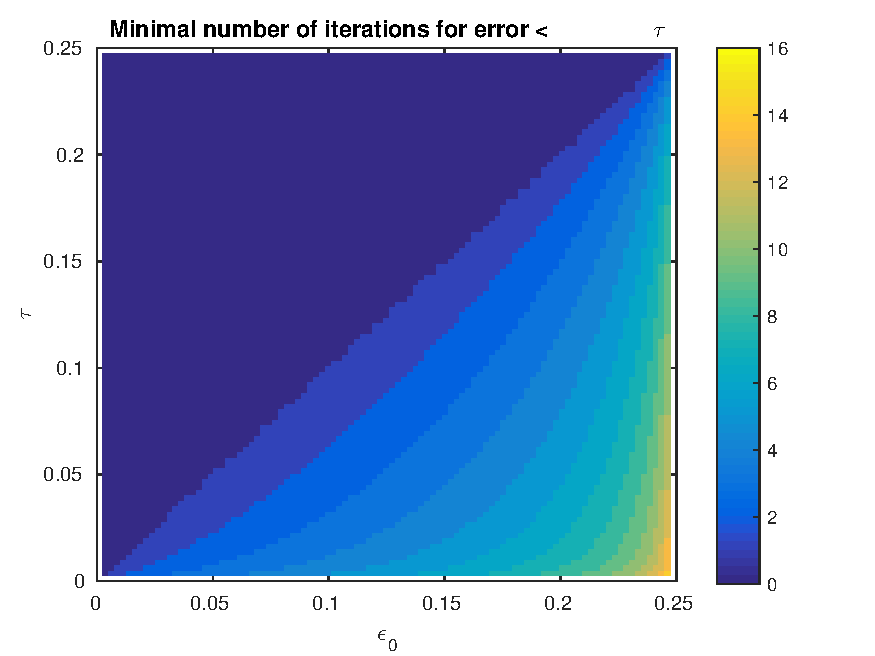
\includegraphics[scale=0.8]{\problems/\chpt/PICTURES/k_min.pdf}
\caption{Minimum number of iterations given $\tau$ and $\epsilon_0$, \ref{prb:ord_p_conv_iter}}
\end{figure}
    \end{solution}

    \end{subproblem}
\end{problem}